\documentclass[10pt,twocolumn]{article}
\usepackage[a4paper, left=1.5cm, right=1.5cm, top=2cm, bottom=3cm]{geometry}
\usepackage[T1]{fontenc}
\usepackage[utf8]{inputenc}
\usepackage[italian]{babel}
\usepackage{amsmath}
\usepackage{titling}
\usepackage{amssymb}
\usepackage{caption}
\usepackage{graphicx}
\usepackage{float}
\usepackage{relsize}
\usepackage{titlesec}
\usepackage{ragged2e}
\usepackage{circuitikz}
\usepackage{booktabs}
\usepackage{longtable}
\usepackage{makecell}
\usepackage{pdflscape}
\usepackage{enumitem}
\usepackage{tikz}
\usepackage{physics}
\usepackage{xcolor}
\usepackage[most]{tcolorbox}
\usepackage{tikz-3dplot}
\usepackage{siunitx}
\usetikzlibrary{decorations.pathmorphing}
\usetikzlibrary{arrows.meta}              % Necessario per l'opzione >=Stealth
\usepackage[colorlinks=true, linkcolor=black]{hyperref}  %per rendere l'indice genrale "interattivo"
\setlist[itemize]{itemsep=4pt, parsep=1pt}
\newtcolorbox{nota}{
  blanker,
  before skip=1em,
  after skip=1em,
  left=1em,
  borderline west={1pt}{0pt}{black},
  fontupper=\itshape,
  before upper={\noindent\textbf{Nota}:\quad}
}

% ---- Suggerimenti su cosa dire nella sezione Grafici ----
% Metti \hintsfalse per nascondere tutti i riquadri \sugg{...}
\newif\ifhints
\hintstrue
\newcommand{\sugg}[1]{%
  \ifhints
  \par\vspace{6pt}\noindent
  \fcolorbox{orange!70!black}{yellow!12}{%
    \parbox{\dimexpr\linewidth-2\fboxsep-2\fboxrule\relax}{\footnotesize\justifying\noindent\textbf{Da dire:} #1}}%
  \par\vspace{8pt}
  \fi}

\setlength{\intextsep}{8pt} % per regolare la distanza grafico tabelle
\setlength{\columnsep}{60pt}
\setlength{\tabcolsep}{4pt}

\begin{document}

    \justifying

      \title{\textbf{Misura dell'angolo di Brewster}}
      \author{Tedeschini Michele \hspace{0.7cm} Stroili Emanuele \hspace{0.7cm} Mirolo Manuele \hspace{0.7cm} Brusini Alessio}
      \date{13 novembre 2026}
      \maketitle
      \newgeometry{left=3cm, right=3cm, top=4cm, bottom=4cm}
      \onecolumn
      \tableofcontents
    \vspace{3cm}
      \begin{abstract}
        \centering
        \large
        L'esperimento consiste nel misurare l'indice di rifrazione del vetro di un prisma tramite la misura dell'angolo di Brewster.

      \end{abstract}

      \newpage
    \restoregeometry
    \twocolumn

\section{Legge fisica}
L'angolo di Brewster $\theta_B$ è l'angolo di incidenza al quale la componente riflessa trasversa magnetica (TM) si annulla completamente. Esso è definito da:
\begin{equation}
    \tan\theta_B = \frac{n_t}{n_i}
    \label{eq:brew}
\end{equation}
dove $n_i$ è l'indice di rifrazione del mezzo incidente e $n_t$ quello del mezzo trasmesso.
Conoscendo l'angolo di Brewster è quindi possibile determinare l'indice di rifrazione $n$ del vetro, con $n_i$ indice di rifrazione dell'aria:
\begin{equation}
    n = n_i \tan\theta_B .
    \label{eq:n}
\end{equation}


    \section{Apparato sperimentale}
  \begin{figure}[H]
  \centering
  \resizebox{\columnwidth}{!}{
\begin{tikzpicture}[
    >=Stealth,
    lbl/.style={font=\small}
]
  \def\thB{57}
  \pgfmathsetmacro{\ai}{90+\thB}   % direzione della sorgente rispetto al prisma
  \pgfmathsetmacro{\ar}{90-\thB}   % direzione del cannocchiale rispetto al prisma
  \coordinate (O) at (0,0);

  % ---------------- goniometro ----------------
  \begin{scope}[shift={(0,-0.6)}]
    \draw[thick, fill=gray!10] (0,0) circle (2.3);
    \foreach \a in {0,10,...,350} {
      \draw[thin] (\a:2.3) -- (\a:2.42);
    }
  \end{scope}

  % ---------------- prisma ----------------
  \draw[thick, fill=cyan!20] (-1.6,0) -- (1.6,0) -- (0,-1.6) -- cycle;
  \node[lbl] at (0,-0.6) {prisma};

  % ---------------- normale e angoli ----------------
  \draw[dashed, thin] (0,0) -- (0,3.7);
  \node[lbl, above] at (0,3.7) {normale};
  \draw[<->, thin] (90:1.25) arc (90:\ai:1.25);
  \draw[<->, thin] (\ar:1.25) arc (\ar:90:1.25);
  \node[lbl] at (118:1.62) {$\theta_B$};
  \node[lbl] at (62:1.62) {$\theta_B$};

  % ---------------- raggio incidente e riflesso ----------------
  \draw[thick, red!70!black, ->] (\ai:5.85) -- (O);
  \draw[thick, red!70!black, ->] (O) -- (\ar:3.6);

  % ---------------- lampada al sodio ----------------
  \begin{scope}[shift={(\ai:6.4)}, rotate=\thB-90]
    \draw[thick, rounded corners=2pt, fill=yellow!35] (-0.55,-0.55) rectangle (0.55,0.55);
  \end{scope}
  \node[lbl, above, align=center] at (-5.6,4.1) {lampada al sodio\\($\lambda = 589$ nm)};

  % ---------------- fenditura ----------------
  \begin{scope}[shift={(\ai:5.0)}, rotate=\thB-90]
    \draw[line width=2pt] (0,-0.42) -- (0,-0.12);
    \draw[line width=2pt] (0,0.12) -- (0,0.42);
  \end{scope}
  \node[lbl, above right] at (-4.0,2.95) {fenditura};

  % ---------------- polarizzatore ----------------
  \begin{scope}[shift={(\ai:3.9)}, rotate=\thB-90]
    \draw[thick, fill=blue!20] (-0.06,-0.55) rectangle (0.06,0.55);
  \end{scope}
  \node[lbl, below left] at (-3.55,1.8) {polarizzatore};

  % ---------------- cannocchiale ----------------
  \begin{scope}[shift={(\ar:3.6)}, rotate=\ar]
    \draw[thick, fill=gray!15] (0.1,-0.4) rectangle (2.4,0.4);
    \draw[thick, fill=gray!35] (2.4,-0.18) rectangle (3.1,0.18);
    \draw[thick, fill=white] (0,0) ellipse (0.1 and 0.5);
    \draw[thick, red!70!black, ->] (0.1,0) -- (3.1,0);
    \draw[thick, fill=white] (3.9,0) circle (0.3);
    \draw[thin] (3.9,-0.3) -- (3.9,0.3);
    \draw[thin] (3.6,0) -- (4.2,0);
  \end{scope}
  \node[lbl, right] at (5.0,1.1) {cannocchiale};
  \draw[->, thin] (5.0,1.2) -- (4.25,2.35);
  \node[lbl, right] at (6.2,2.5) {oculare};
  \draw[->, thin] (6.2,2.55) -- (5.5,3.35);
  \node[lbl, right] at (6.9,4.55) {mirino};
  \draw[->, thin] (6.9,4.5) -- (6.4,4.15);

  % ---------------- etichette goniometro e prisma ----------------
  \node[lbl, left, align=right] at (-2.6,-2.9) {goniometro ottico};
  \draw[->, thin] (-2.6,-2.9) -- (-1.75,-2.3);
  \node[lbl, right, align=center] at (3.0,-1.3) {faccia più grande\\del prisma};
  \draw[->, thin] (3.0,-1.2) -- (1.0,-0.05);

\end{tikzpicture}
 }
\end{figure}
  

L'apparato per misurare l'angolo di Brewster è composto da:
\begin{itemize}
    \item Una lampada al sodio ($\lambda = 589$ nm), con una fenditura che definisce il fascio di luce.
    \item Un polarizzatore, posto sul cammino del fascio incidente, ruotato in modo da lavorare in polarizzazione TM.
    \item Un goniometro ottico su cui è appoggiato il prisma di vetro: dove si misura la luce riflessa.
    \item Un cannocchiale con mirino, che permette di seguire il raggio riflesso e di leggerne la posizione.
\end{itemize}

\section{Analisi Dati}
    Per misurare l'angolo di Brewster si è misurata la posizione di zero $\theta_0$ del goniometro (senza il prisma) e la lettura $\theta_i$ del cannocchiale in corrispondenza del raggio riflesso, ricavando
    \begin{equation}
        \theta_B = \frac{\pi - |\theta_i - \theta_0|}{2}.
        \label{eq:thB}
    \end{equation}
    L'incertezza sulla singola misura è difficile da stimare a priori, quindi la misura è stata ripetuta riposizionando ogni volta prisma e cannocchiale: in totale 105 misure di 4 persone diverse (Tab.~\ref{tab:dati}).

    \noindent Dalle misure otteniamo:
    \begin{itemize}
      \item L'istogramma dei valori di $\theta_B$ per ciascuna persona e per tutti i dati. Si proverà a descriverlo tramite una gaussiana di parametri $\mu$ e $\sigma$. 
      Non ci attendiamo però che la distribuzione sia necessariamente gaussiana: gli errori cadono prevalentemente dal lato in cui l'intensità della luce varia lentamente, quindi la distribuzione può risultare asimmetrica.

      \item La media, la deviazione standard e l'incertezza sulla media di $\theta_B$, per ciascuna persona e per tutti i dati:
      \begin{equation}
        \bar\theta_B = \frac{1}{N}\sum_{i=1}^{N}\theta_{B,i} \qquad \sigma_{\bar\theta_B} = \frac{\sigma_{\theta_B}}{\sqrt{N}}
        \label{eq:stat}
      \end{equation}

      \item L'indice di rifrazione $n = n_i\tan\bar\theta_B$, con $n_i = 1{,}000293$ indice dell'aria, e la sua incertezza (con $\sigma_{\bar\theta_B}$ in radianti):
      \begin{equation}
    \sigma_n = \frac{n_i}{\cos^2\bar\theta_B}\,\sigma_{\bar\theta_B}        \label{eq:sigman}
      \end{equation}

      \noindent Se la misura è corretta ci aspettiamo che i valori di $n$ delle diverse persone siano compatibili tra loro e con $n_{\mathrm{Sell}} = 1{,}5285 \pm 0{,}0003$, ricavato con il modello di Sellmeier nell'esperienza 3. 
      Si ha la compatibilità quando lo scarto soddisfa
      \begin{equation}
        |n - n_{\mathrm{Sell}}| \leq 2\sqrt{\sigma_n^2 + \sigma_{\mathrm{Sell}}^2}
        \label{eq:comp}
      \end{equation}
      
    \end{itemize}


  \section{Grafici}
    Si riportano i grafici e le tabelle ottenuti.

       \begin{figure}[H]
        \centering
      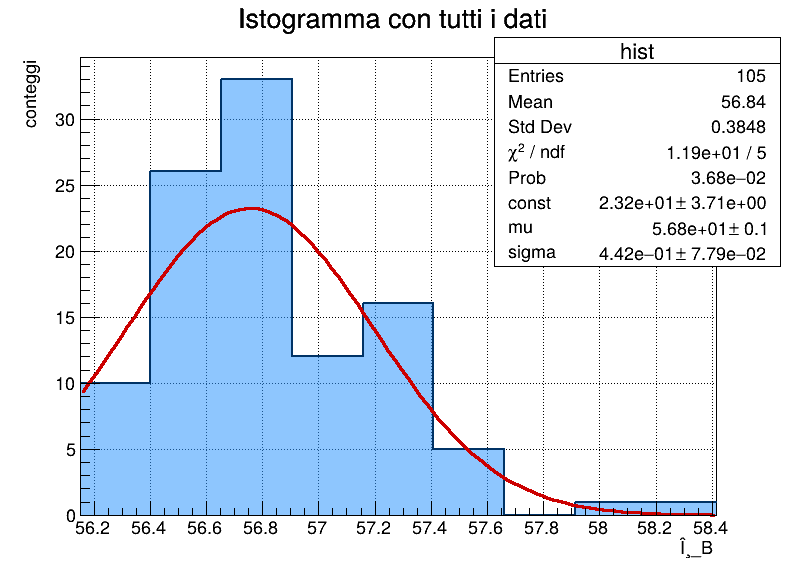
\includegraphics[width=1.0\columnwidth]{Immagini/hist_totalData.png}
        \caption{Istogramma di tutte le misure di $\theta_B$ ($N = 105$) con fit gaussiano.}
        \label{fig:hist_tot}
      \end{figure}




\noindent Come si può vedere dall'istogramma complessivo di tutte le 105 misure esso non si distribuisce secondo una gaussiana, ciò è dovuto sall'andamento dell'intensità luminosa: essa aumentava fin da subito la propria intensità per angoli cresecnti rispetto al valore dell'angolo in cui essa sia annullava. Proprio per questo motivo non ci aspetta dunque un andamento gaussiano ma uno che è ricondicibile  a quest'ultimo per valori di angoli osservati minori dell'angolo di Brewster medio e un "troncamento" della coda per angoli cresecnti:


      \begin{figure}[H]
        \centering
      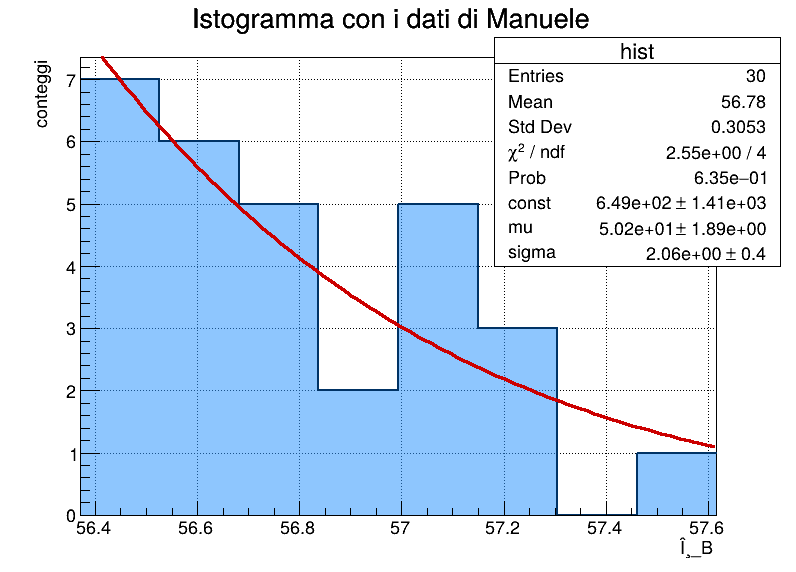
\includegraphics[width=1.0\columnwidth]{Immagini/histManuData.png}
        \caption{Istogramma delle misure di $\theta_B$ di Manuele ($N = 30$) con fit gaussiano.}
        \label{fig:hist_manu}
      \end{figure}

      \begin{figure}[H]
        \centering
      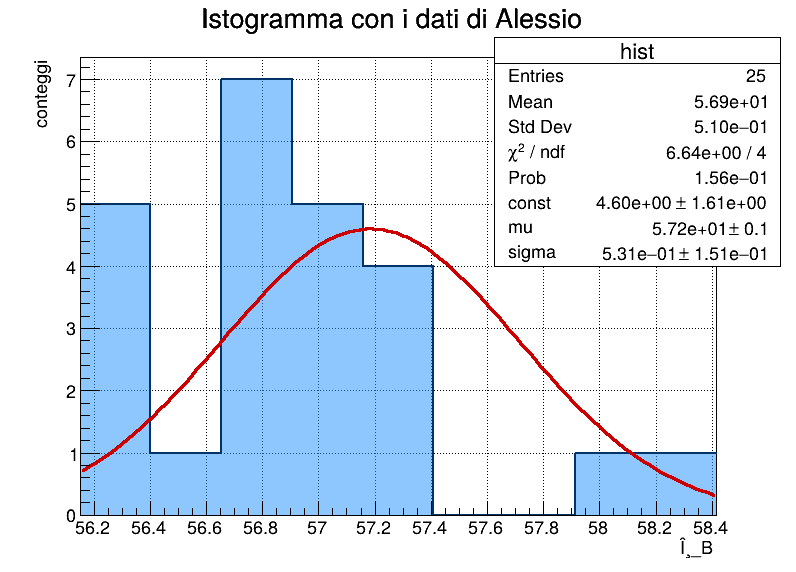
\includegraphics[width=1.0\columnwidth]{Immagini/histAleData.png}
        \caption{Istogramma delle misure di $\theta_B$ di Alessio ($N = 25$) con fit gaussiano.}
        \label{fig:hist_ale}
      \end{figure}

      \begin{figure}[H]
        \centering
      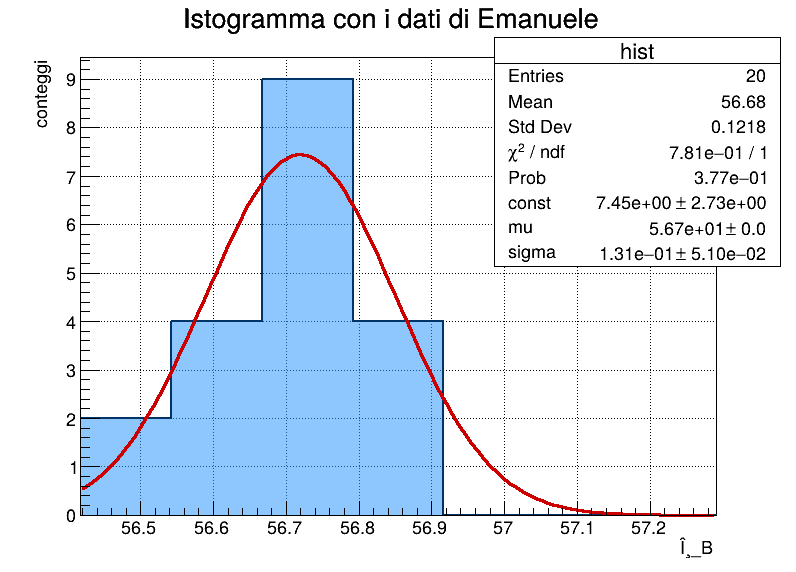
\includegraphics[width=1.0\columnwidth]{Immagini/histStroiliData.png}
        \caption{Istogramma delle misure di $\theta_B$ di Emanuele ($N = 20$) con fit gaussiano.}
        \label{fig:hist_stroili}
      \end{figure}

      \begin{figure}[H]
        \centering
      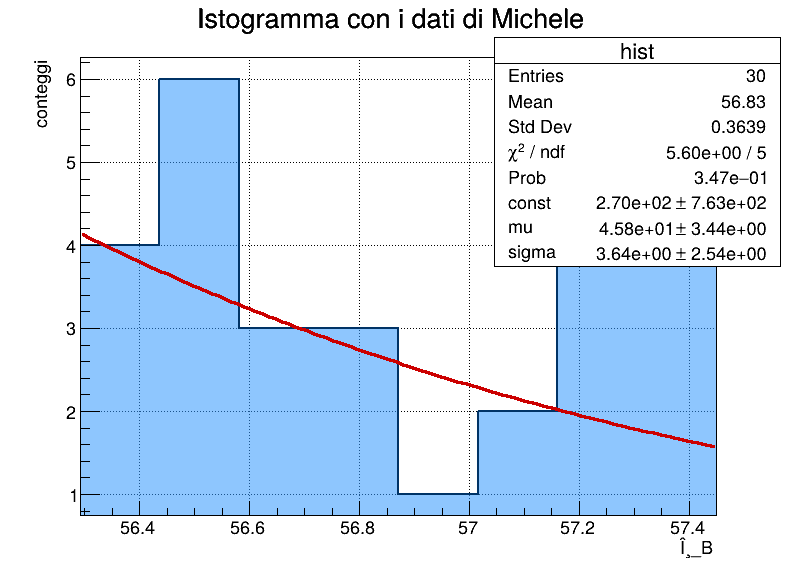
\includegraphics[width=1.0\columnwidth]{Immagini/histMichData.png}
        \caption{Istogramma delle misure di $\theta_B$ di Michele ($N = 30$) con fit gaussiano.}
        \label{fig:hist_mich}
      \end{figure}



\textbf{DA DIRE: ogni persona ha media e dispersione diverse a causa della sensibilità divers inoltre con pochi dati il fit gaussiano ha poco significato}
Analizzando la distribuzione di ciascun osservatore si può dedurre che: per il primo e il quarto osservatore l'istogramma non si distribuisce secondo nessuna distribuzione nota, nonostante ciò i valori medi ricavati risultano essere compatibili tra di loro e risultano essere compatibili con il valore medio ricavato dalla distribuzione del secondo osservatore. La non compatibilità avviene con il valore medio del terzo osservatore: si può notare che la discrepanza tra il valore della scarto tra i valori medi e il valore di soglia per la compatibilità è dell'ordine del millesimo di grado; rispettivamente tra il secondo e il terzo osservatore è pari a $0,0014$° e tra il terzo e il quarto è di $0,0066$°. 
Infine, soffermandosi sulle distribuzioni dei singoli osservatori, è importante far notare che in mancanza di un campione di dimensioni adeguatamente estese non ha particolare signifcato esguire un fit con una normale standard.

      \begin{table}[H]
        \centering
        \small
        \begin{tabular}{lcccc}
          \toprule
          Persona & $N$ & $\bar\theta_B$ [$^\circ$] & $\sigma_{\theta_B}$ [$^\circ$] & $\sigma_{\bar\theta_B}$ [$^\circ$] \\
          \midrule
          Manuele & $30$ & $56{,}811$ & $0{,}34$ & $0{,}062$ \\
          Alessio & $25$ & $56{,}97$ & $0{,}59$ & $0{,}12$ \\
          Emanuele & $20$ & $56{,}715$ & $0{,}18$ & $0{,}041$ \\
          Michele & $30$ & $56{,}889$ & $0{,}40$ & $0{,}073$ \\
          \midrule
          Totale & $105$ & $56{,}853$ & $0{,}41$ & $0{,}040$ \\
          \bottomrule
        \end{tabular}
        \caption{Media, deviazione standard e incertezza sulla media di $\theta_B$ per ciascun persona e per tutti i dati.}
        \label{tab:theta}
      \end{table}



      \texttbf{DA DIRE: le medie delle quattro persone differiscono di pochi decimi di grado}
      
        \begin{table}[H]
        \centering
        \footnotesize
        \setlength{\tabcolsep}{1.5pt}
        \begin{tabular}{lcccc@{\hspace{3pt}}c}
          \toprule
          Persona & $n$ & $\sigma_n$ & $|n - n_{\mathrm{Sell}}|$ & $2\sqrt{\sigma_n^2 + \sigma_{\mathrm{Sell}}^2}$ & \makecell{compati-\\bilità} \\
          \midrule
          Manuele & $1{,}5292$ & $0{,}0036$ & $0{,}00076$ & $0{,}00728$ & sì \\
          Alessio & $1{,}5387$ & $0{,}0070$ & $0{,}01022$ & $0{,}01392$ & sì \\
          Emanuele & $1{,}5236$ & $0{,}0024$ & $0{,}00482$ & $0{,}00476$ & no \\
          Michele & $1{,}5338$ & $0{,}0043$ & $0{,}00536$ & $0{,}00855$ & sì \\
          \midrule
          Totale & $1{,}5317$ & $0{,}0024$ & $0{,}00325$ & $0{,}00475$ & sì \\
          \midrule
          $n_{\mathrm{Sell}}$ & $1{,}5285$ & $0{,}0003$ & -- & -- & -- \\
          \bottomrule
        \end{tabular}
        \caption{Indici di rifrazione e verifica della compatibilità}
        \label{tab:n}
      \end{table}
      Riportiamo infine la tabella dei valori degli indici di rifrazione ricavati dal campione complessivo delle 105 misure e dal campione del singolo osservatore:


      \begin{figure}[H]
        \centering
      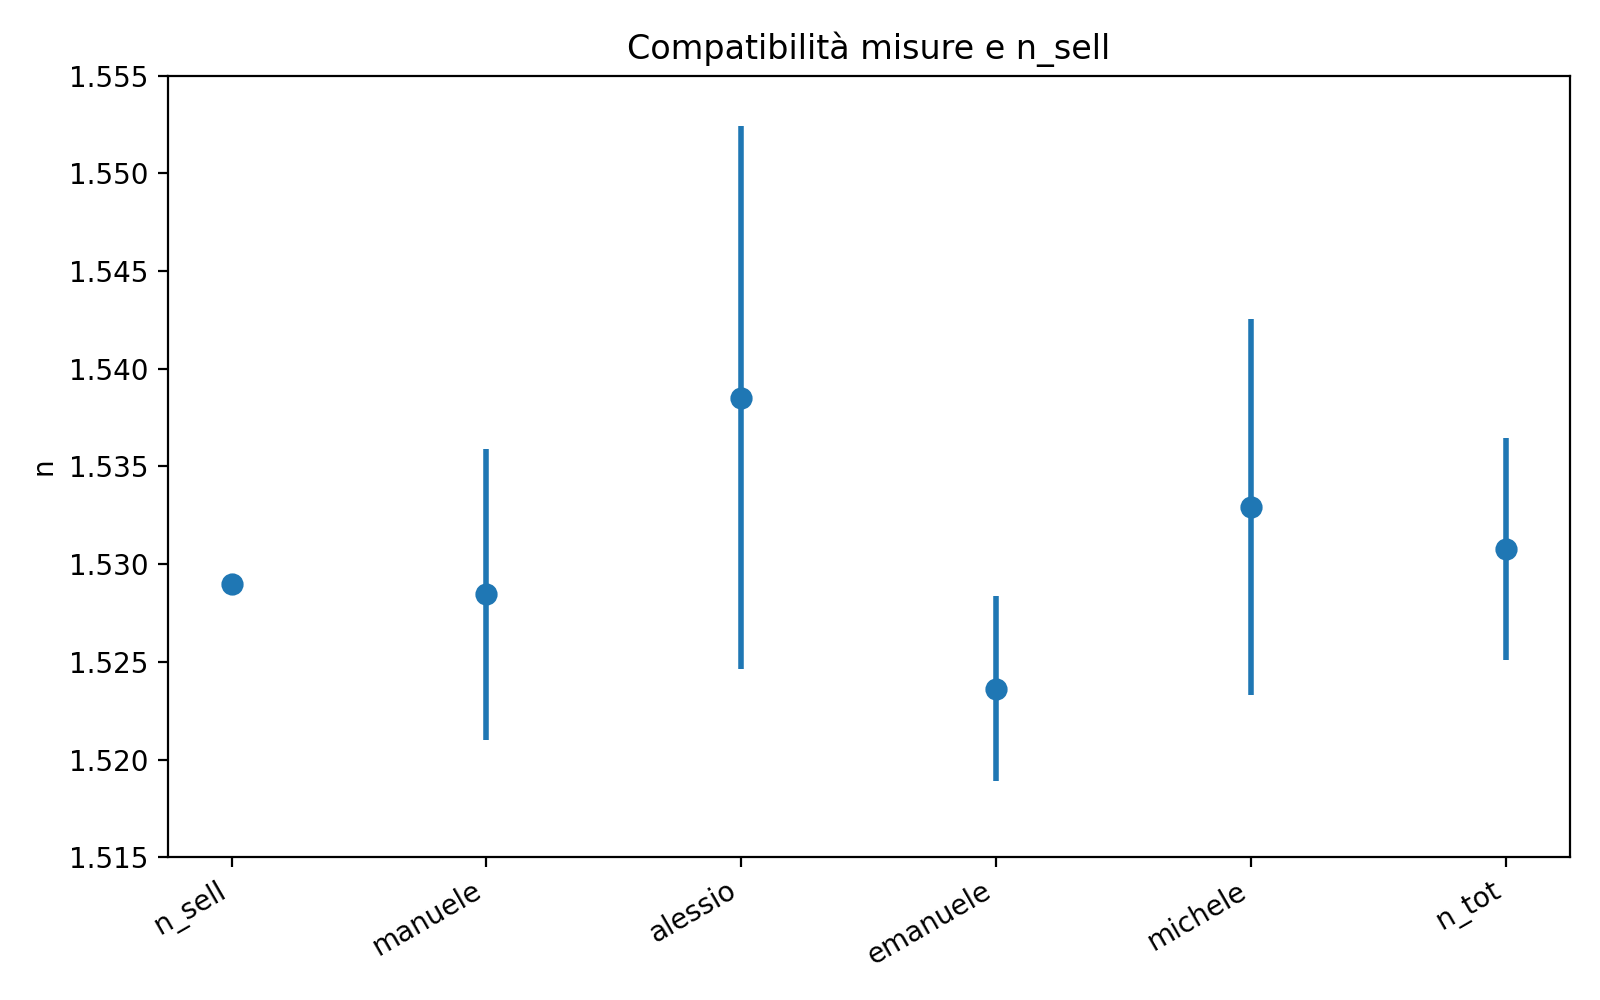
\includegraphics[width=1.0\columnwidth]{Immagini/pointrange.png}
        \caption{Indice di rifrazione $n$ per ciascuna persona e per tutti i dati, confrontato con $n_{\mathrm{Sell}}$ dell'esperienza 3.}
        \label{fig:pointrange}
      \end{figure}

      \textbf{DA DIRE: 3 valori su 4 sono compatibili con n di sellmeir poi la precisione è peggiore rispetto l'esperienza 3 come ci si aspetta e restano errori sistematici che non si possono togliere tipo sensibilità persone che fanno spostare il minimo e la disomogeneta polarizzatore}
      Dai valori sopra riportati e dal grafico di \fig{6} possiamo constatare che: le misure dell'indice di rifrazione risultano compatibili tra di loro sia ytra coascun osservatore sia quella del singolo con il valore medio estartto dal campione complessivo, in secondo luogo la compatibilità con il valore dell'indice di rifrazione misurato nella precedente esperienza di laboratorio avviene per tre osservatori su quattro: una possibile fonte d'errore in cui è facile imbattersi nello svolgimento di questa misura è la sensibilità all'intensità luminosa di chi osserva, che è soggetiva. Per quanto riguarda il valore ottenuto prendendo in cosiderazione il campione complessivo ci aspettava la compatibilità poichè aumenntando il numero di misure il valore medio tende a quello più probabile (devo rilegeere sono di fertta sta andando a lezioen) 




      \section{Conclusioni}


\onecolumn
\begin{table}[!t]
\centering
\begin{tabular}{ccccc}
\toprule
$i$ & Manuele & Alessio & Emanuele & Michele \\
\midrule
1 & 56.625 & 58.417 & 56.667 & 56.450 \\
2 & 57.083 & 56.717 & 56.875 & 57.325 \\
3 & 56.517 & 56.400 & 56.750 & 56.700 \\
4 & 57.617 & 56.183 & 56.825 & 56.783 \\
5 & 57.117 & 58.242 & 56.667 & 56.525 \\
6 & 56.583 & 56.183 & 56.825 & 57.450 \\
7 & 57.017 & 56.817 & 56.875 & 57.450 \\
8 & 56.700 & 57.150 & 57.292 & 56.567 \\
9 & 56.450 & 57.233 & 56.633 & 56.292 \\
10 & 56.892 & 56.900 & 56.617 & 56.400 \\
11 & 57.292 & 56.325 & 56.667 & 57.125 \\
12 & 56.575 & 57.292 & 56.667 & 56.333 \\
13 & 56.450 & 57.067 & 56.667 & 56.367 \\
14 & 56.533 & 58.042 & 56.733 & 57.200 \\
15 & 56.700 & 56.150 & 56.783 & 56.767 \\
16 & 56.450 & 56.708 & 56.733 & 56.450 \\
17 & 56.892 & 56.550 & 56.558 & 56.900 \\
18 & 56.450 & 57.150 & 56.417 & 57.200 \\
19 & 56.508 & 56.667 & 56.542 & 56.567 \\
20 & 57.200 & 57.142 & 56.500 & 56.567 \\
21 & 56.700 & 56.875 &  & 57.375 \\
22 & 57.200 & 56.717 &  & 57.033 \\
23 & 57.100 & 57.167 &  & 57.367 \\
24 & 56.742 & 56.967 &  & 57.250 \\
25 & 56.783 & 57.250 &  & 57.450 \\
26 & 57.075 &  &  & 56.700 \\
27 & 56.370 &  &  & 56.650 \\
28 & 56.533 &  &  & 57.408 \\
29 & 57.550 &  &  & 57.300 \\
30 & 56.617 &  &  & 56.733 \\
\bottomrule
\end{tabular}
\caption{Misure di $\theta_B$ [gradi] di ciascuna persona.}
\label{tab:dati}
\end{table}
\end{document}
